\documentclass[oneside,senior,etd]{BYUPhysForDegree}

\usepackage[utf8]{inputenc}
\usepackage{rotating} 

\usepackage[russian]{babel}
\usepackage{amsfonts}
\usepackage{amstext}
\usepackage{amssymb}
\usepackage{amsthm}
\usepackage{graphicx}
\usepackage{subfig}
\usepackage{color}
\usepackage[unicode]{hyperref}
\usepackage[nottoc]{tocbibind}
\usepackage{algorithmic}
\usepackage{algorithm}
\usepackage{verbatim}
\usepackage{listings}

\usepackage{commath}
\newcommand\Tau{\mathcal{T}}
\newcommand{\R}{\mathbb{R}}
\usepackage{color}
\usepackage[colorinlistoftodos, prependcaption]{todonotes}
\usepackage{multirow}
\newcommand*{\MyIndent}{\hspace*{0.2cm}}

\Chair{Кафедра Системного Программирования}
\Lab{~}
\Year{2020}
  \Month{Май}
  \City{Москва}
  \AuthorText{Автор}
  \Author{Фомин Сергей Александрович}
  \AuthorEng{}
  \AcadGroup{328}
  \TitleTop{Исследование методов быстрого поиска изображений}
  \TitleBottom{ в задаче распознавания лиц}
  \TitleTopEng{Research methods for fast image search}
  \TitleBottomEng{in the face recognition problem} 
  \docname{Курсовая работа}
  \Advisor{Архипенко Константин Владимирович}
  \Consultant{Рындин Максим Алексеевич}
  
\Abstract{Одной из востребованных областей поиска с Интернете является поиск по изображениям. Современные методы индексации данных показывают отличный результат поиска в многомиллиардных коллекциях и повсеместно применяются для данной задачи. В этой работе предлагается изучить существующие подходы индексации большого количества изображений и посмотреть на поведение этих алгоритмов в задаче распознавания лиц. Будем считать, что современные нейросетевые алгоритмы достаточно хорошо выделяют признаки лица на изображении, и лишь немного затронем этот вопрос. Основной задачей ставим сравнение скорости поиска индексных методов на наборах данных лиц. Начнем рассмотрение с простейших алгоритмов поиска, таких как поиск по точному расстоянию и простая индексная структура. Затем на более продвинутых алгоритмах увеличим скорость поиска и исследуем ухудшение точности. Эксперименты показывают, что в больших коллекция изображений лиц можно добиться приемлемой скорости поиска с хороших показателем точности. Сильное же ускорение приводит к большим потерям.}
\AbstractEng{Abstract}


\University{Московский государственный университет имени М.В.Ломоносова}
\Faculty{Факультет вычислительной математики и кибернетики}
\GrText{гр.}
\AdvisorText{Научный руководитель}
\ConsultantText{Научный консультант}
\AbstractText{Аннотация}

\begin{document}
\fixmargins

\makepreliminarypages

\oneandhalfspace

\tableofcontents

\section*{Введение}
\addcontentsline{toc}{section}{Введение}
\label{sec:Chapter0} \index{Chapter0}


В последнее десятилетие визуальный поиск стал широко распространенной функцией многих поисковых систем. Большой объем сохраненных изображений в сети измеряется петабайтами, число которых с каждым днем только увеличивается. В связи с этим эффективный поиск ближайших соседей является серьезной исследовательской проблемой~\cite{1,2,3,4,5,6}. Потребность быстрого поиска похожих изображений занимает большую нишу в современных приложениях компьютерного зрения, в том числе в задаче распознавания лиц~\cite{8}. Социальные сети, правоохранительные органы имеют огромные коллекции изображений лиц, среди которых надо уметь быстро извлекать нужную информацию. Для решения данной проблемы требуются эффективные и масштабируемые алгоритмы поиска с низкими временными затратами. Ожидается, что ответ на запросы к базам данных из миллиардов элементов будет занимать несколько миллисекунд.

Решение данной задачи можно рассматривать с двух сторон. Во-первых, даже самые современные алгоритмы поиска и обработки лиц на изображении не идеальны. Это открывает просторы для исследований. Во-вторых, подходящая структура данных для поиска может давать многократное увеличение скорости. Среди всех алгоритмов распознавания сверточные нейронные сети (CNN) показывают лучшие результаты поиска лиц на изображении и используются в большинстве исследованиях этой области \cite{8,10}. В связи с этим основной задачей исследования будем считать проблему выбора поисковой структуры данных, а дескрипторы лиц для экспериментов будем строить по одной из общедоступных CNN. 

Все существующие крупномасштабные поисковые системы избегают исчерпывающего поиска путем ограничения конечного набора кандидатов, который рассматривается для запроса. Данный подход называют приближенным поиском ближайших соседей (ANN). Современные алгоритмы ANN имеют три основных реализации: инвертированная индексация~\cite{1,2,3,4,5,6}, хеширование~\cite{9}, многомерная инвертированная индексация, основанная на квантовании произведения (PQ)~\cite{4,5}. В этой работе основное внимание уделено инвертированному индексу и его оптимизации с помощью PQ.

Структуры индексации разбивают пространство поиска на большое количество непересекающихся областей, и в процессе поиска используется только малая часть коллекции, наиболее близкая к конкретному запросу. Отобранная часть данных образует короткий список кандидатов, и поисковая система рассчитывает расстояния между запросом и всеми кандидатами. На этом этапе важно, чтобы список кандидатов был коротким, так как вычисление расстояния имеет линейную сложность по данной длине. Метод PQ для ANN используется в двух видах: для построения многомерного инвертированного индекса для приближенного поиска или для кодирования векторов в компактные коды для точного поиска. Идея этих подходов состоит в том, чтобы разложить пространство векторов на большое количество непересекающихся множеств и обучить запросы получать доступ к ближайшим из них.

Первая структура индексации, способная работать с миллиардным набором данных, представлена в~\cite{1}. Она основана на структуре инвертированного индекса, которая разбивает пространство признаков на диаграмму Вороного. Каждая область задается своим центроидом, который предварительно обучили алгоритмом $K$-средних. Показано, что эта система достигает разумных скоростей поиска, порядка нескольких десятков миллисекунд. Позже обобщение структуры инвертированного индекса предложили в~\cite{3}. В этой работе представлен инвертированный многомерный индекс или мульти-индекс (IMI), который разбивает пространство признаков на несколько ортогональных подпространств, и каждое подпространство обучается независимо друг от друга. Декартово произведение такого разбиения образует неявное разбиение всего пространства поиска. Обе эти структуры обладают своими недостатками, которые можно устранить с помощью различных оптимизаций PQ~\cite{6,7}.

В данной работе описано несколько современных архитектур индексирования, и путем экспериментов исследована их применимость к задаче распознавания лиц. % Введение
\section{Постановка задачи}
\label{sec:Chapter1} \index{Chapter1}

Главной задачей данной работы является исследование современных индексных структур быстрого поиска и поверка их эффективности в задаче распознавания лиц. Считается, что выделением лица на изображении и построением его признаков занимаются алгоритмы общедоступных сверточных нейронных сетей. Работа производится в рамках построенных 128-мерных векторов, по одному для каждого изображения. Время построения каждого вектора учитывать не будем, так как во всех алгоритмах будет использоваться одна и та же нейронная сеть. Также не будем учитывать, но обратим внимание на время обучения индексных структур, так как для разных алгоритмов оно может отличаться на порядки.

Проверка заключается в измерении среднего времени поиска похожих лиц в большой коллекции изображений. Время, затраченное на поиск $K$ ($K = 1, 5, 10, 30, 50, 100$) ближайших соседей является основным критерием скорости алгоритма. Помимо скорости важно учитывать точность поиска. Во всех сопутствующих работах \cite{1,3,5,6,7} точность измеряется как процент истинных ближайших соседей среди $K$ найденных, где истинные ближайшие соседи определяются точным евклидовым расстоянием. Использовать данную метрику в этой работе следует аккуратно, так как она не отражает природы исследуемой области, а указывает только лишь на качество используемого алгоритма, который и без того много лет тестируется и улучшается. В связи со спецификой нашей задачи, наиболее правильным вариантом измерения точности будет получение процента лиц, отмеченных так же, как и запрос, среди $K$ найденных ближайших соседей. Также в качестве альтернативного показателя качества будем измерять частоту вхождения каждого лица в $K$ ближайших соседей. В случае совпадения лица запроса и лица с наибольшей частотой будем говорить об успешном распознавании. Во многих задачах распознавания образов используется именно эта метрика.

Для применимости данного подхода к реальным задачам алгоритм должен удовлетворять нескольким требованиям:
\begin{enumerate} 
\item Скорость поиска в большом объеме изображений не должна превышать нескольких миллисекунд;
\item Точность поиска должна быть в пределе допустимой для выбранного алгоритма, то есть не сильно отличаться от приводимой в статьях.
\end{enumerate} 

В качестве вывода следует оценить показатели точности и скорости распознавания лиц на основе результатов экспериментов, а также сформулировать возможные пути улучшения.
 % Постановка задачи
\section{Обзор существующих решений}
\label{sec:Chapter2} \index{Chapter2}

В данной части работы кратко описаны несколько идей из существующих работ и попутно введены обозначения для дальнейшего исследования.
Начнем с того, что во всех упомянутых ниже алгоритмах решается одна и та же задача. А именно, вычисление евклидовых расстояний между векторами высокой размерности.

Рассмотрим $D$-мерное евклидово пространство $R^D$. Общая задача состоит в том, чтобы найти элемент  $NN(x)$ в конечном наборе $Y\subset R^D$, минимизируя расстояние до вектора запроса $x\in R^D$: 
$$NN(x) = \underset{y\in Y}{\operatorname{argmin}}(d(x, y)).$$
Поиск ближайшего соседа по своей природе дорогой из-за влияния высокой размерности дескрипторов. Для сокращения времени поиска предложено несколько методов многомерного индексирования, таких как популярное $KD$-дерево или другие методы ветвей и границ. Однако для больших размерностей оказывается, что такие подходы не намного эффективнее, чем исчерпывающий расчет расстояний~\cite{12}, сложность которого составляет $O(ND)$. Также одним из самых популярных алгоритмов ANN является евклидово локально-чувствительное хеширование (LSH)~\cite{9}. Однако наивный подход к реализации данного метода не учитывает требования к памяти структуры индексации~\cite{2}. В LSH использование памяти может оказаться даже выше, чем у исходных векторов. Этот факт, а также факт наличия случайности серьезно ограничивают применимость данного алгоритма.

\begin{figure}[h]
\begin{minipage}[h]{0.48\linewidth}
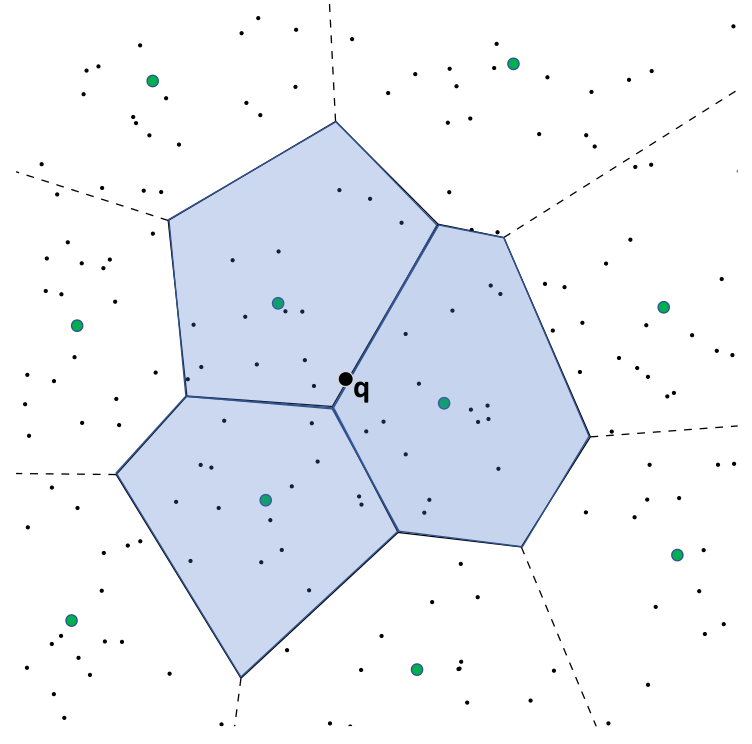
\includegraphics[width=1\linewidth]{Images/Index.png}
\caption{Индексная структура. Зеленым цветом обозначены центроиды ячеек. Черная точка $q$ — запрос поиска. Синим цветом выделены ближайшие ячейки, вектора которых попадают в список кандидатов.}
\label{ris:index}
\end{minipage}
\hfill
\begin{minipage}[h]{0.48\linewidth}
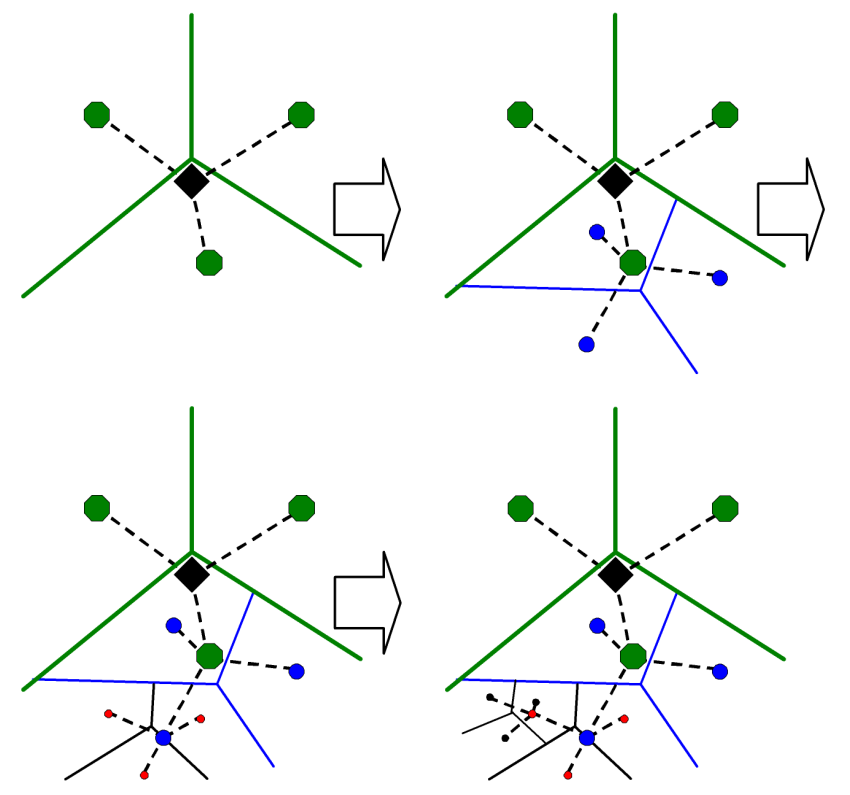
\includegraphics[width=1\linewidth]{Images/HierarchicalIndex.png}
\caption{Иерархический индекс. Процесс построения иерархического инвертированного индекса с разбиением на $K$ ячеек ($K$ = 3). На рисунке представлено четырехуровневое разбиение.}
\label{ris:hierachicalindex}
\end{minipage}
\end{figure}

В связи с этим более подробно обсудим алгоритмы индексирования, основанные на квантовании. Так как полное сравнение вектора запроса со всеми векторами коллекции невозможно, список кандидатов нужно сокращать. Поэтому была придумана инвертированная индексная структура для быстрого доступа к наиболее значимым векторам. Общая идея в том, что инвертированый индекс содержит связные списки векторов, где каждый список является отображением некоторого вектора-центроида. На первом этапе запроса определяется центроид, затем по определенному этим вектором списку выполняется исчерпывающий поиск (Рис.~\ref{ris:index}).

Простейший инвертированный индекс основан на векторном квантовании (VQ)~\cite{1,2,7}. Цель VQ -- уменьшить количество элементов представления пространства поиска. Формально VQ -- это функция $q$, отображающая $D$-мерный вектор $x\in R^D$ на вектор $q(x)\in C = \{c_i~|~i\in I\}$, где $I$ -- конечное индексное множество: $I = 0 , ... , k-1$. Вектора $c_i$ называются центроидами. Множество $V_i$ векторов, отображаемых в данный кластер с номером $i$, называется ячейкой Вороного и определяется так:
$$V_i = \{x\in R^D~|~q(x)=c_i\}.$$
Ячейки VQ образуют разбиение пространства поиска. Все векторы, лежащие в одной и той же ячейке $V_i$, представляются одним и тем же центроидом $c_i$. Качество VQ обычно измеряется по среднеквадратичной ошибке между вектором запроса $x$ и его значением $q(x)$:
$$MSE(q) = \mathbb{E}~d(q(x), x)^2,$$
где $d(x, y) = \| x - y \|$ -- евклидово расстояние между $x$ и $y$.
Стандартным методом обучения центроидов VQ является алгоритм кластеризации $K$-средних, который находит оптимальное разбиение путем итеративного сопоставления векторов центроидам и перестройки этих центроидов по сопоставленным векторам.

Поиск по данной структуре производится в два этапа:
\begin{enumerate}
\item Поиск ближайшего к запросу центроида по короткому списку центроидов;
\item Поиск по списку кандидатов, соответствующих этому центроиду.
\end{enumerate}

\begin{figure}[h]
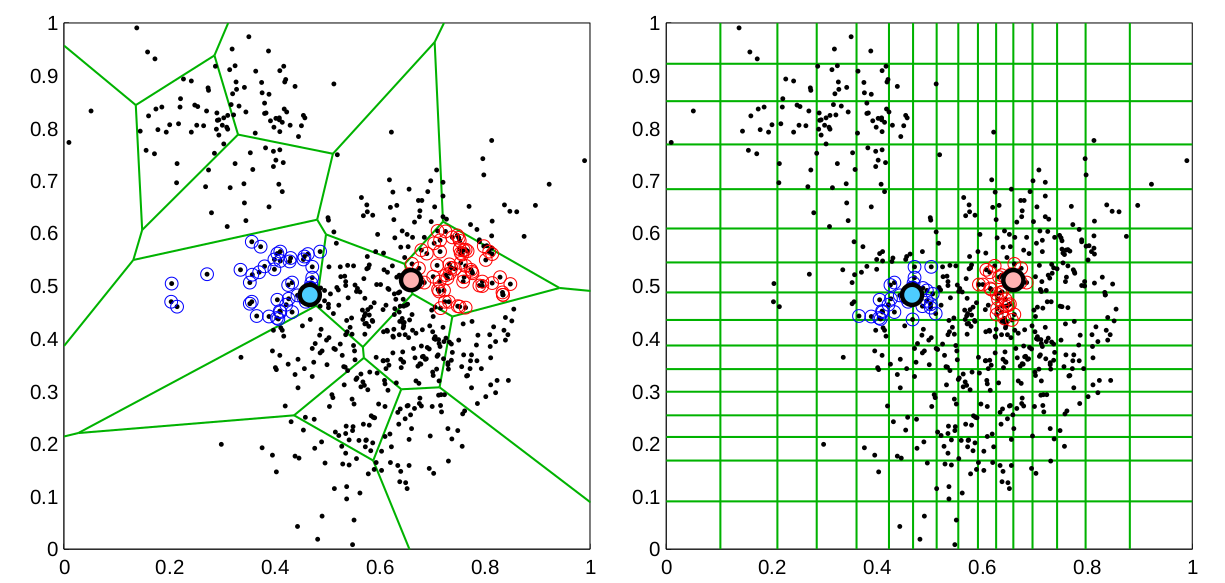
\includegraphics[width=1\linewidth]{Images/MultiIndex.png}
\caption{Левый -- инвертированный индекс. Правый -- инвертированный мульти-индекс. На рисунках представлена разница в разбиении одного и того же набора данных из 600 векторов для разных структур. Для наглядности размерности векторов равны двум. Обе структуры разбивались на 16 ячеек (для каждой размерности). Для примера обозначим два запроса к базе данных, которые отмечены синим и красным цветом. На левом рисунке списки кандидатов содержат 45 и 62 вектора соответственно. Обратим внимание, когда запрос лежит вблизи границы, список кандидатов получается «перекошенным». Для тех же запросов к мульти-индексной структуре списки получаются короче -- 31 и 32 вектора соответственно. Это связанно с тем, что каждая ячейка содержит меньшее количество векторов. Выбирая несколько близких ячеек, можно добиться более точного списка кандидатов.}
\label{ris:multiindex}
\end{figure}

Чтобы обеспечить высокую скорость поиска с использованием инвертированного индекса, количество ячеек должно быть достаточно велико, что сильно снижает скорость обучения алгоритма на больших объемах данных.

Повысить эффективность этапа обучения можно с помощью инвертированного иерархического индекса (HKM)~\cite{11}, который помимо первичного разбиения на ячейки Вороного разбивает пространство каждой ячейки повторно (Рис.~\ref{ris:hierachicalindex}). В огромных датасетах уровень вложенности разбиения выбирается достаточно большим, что гарантирует небольшой список кандидатов. Помимо скорости обучения, при правильном подборе параметров можно добиться ускорения поиска~\cite{11}.

Еще одна идея использования индексов для быстрого поиска предлагает разбивать пространство векторов на несколько подпространств меньшей размерности и обучать каждое подпространство малой размерности отдельно. Это позволяет разбивать датасет на огромное количество ячеек и с помощью декартова произведения центроидов быстро получать доступ к ним (Рис.~\ref{ris:multiindex}). Данная структура называется инвертированным мульти-индексом (IMI)~\cite{3}.

Более формально IMI основан на квантовании произведения (PQ)~\cite{2}, которое представляет из себя схему сжатия с потерями. PQ кодирует каждый вектор $x\in R^D$ как объединение $M$ $\frac{D}{M}$-мерных центроидов из списков $C_1,..., C_M$, каждый из которых содержит $K$ кодовых слов. Другими словами, PQ разбивает вектор на $M$ отдельных подвекторов и применяет векторное квантование (VQ) к каждому подвектору, используя при этом отдельный список центроидов. Следовательно процесс обучения IMI схож с процессом обучения обычного инвертированного индекса, за тем лишь исключением, что обучать приходится несколько списков центроидов. В результате каждый вектор $x$ кодируется набором индексов $[i_1,..., i_M]$ и аппроксимируется как $x \approx [C_1 (i_1),...,C_M (i_M)]$. Быстрое вычисление евклидова расстояния становится возможным благодаря эффективному асиметричному вычислению расстояния~\cite{2} с использованием обученных центроидов:
$$\|x - y\|^2 \approx \|x - [C_1 (i_1),..., C_M(i_M)]\|^2 = \sum_{m=1}^M\|x_m - C_m(i_m)\|^2,$$
где $x_m$ -- составляющая $m$-го подпространства вектора $x$. С точки зрения геометрии PQ эффективно разделяет исходное векторное пространство на $K^M$ ячеек, каждая из которых является декартовым произведением $M$ ячеек меньшей размерности. Однако стоит учитывать, что из-за огромного количества кластеров в IMI некоторые области могут содержать сравнительно малое количество кандидатов или не содержать совсем. Следовательно, IMI в процессе поиска тратит много времени на посещение пустых областей. Причина этого недостатка состоит в том, что IMI при обучении не учитывает зависимость подпространств, которые зачастую зависимы на практике. В частности, существуют значительные корреляции между различными подпространствами дескрипторов, построенных с помощью сверточных нейронных сетей, которые наиболее актуальны в наши дни. Для решения проблемы адаптации алгоритмов к коррелированным данным можно предварительно производить ортогональные преобразования над данными~\cite{4,6} или локальные оптимизации PQ~\cite{5}. % Обзор существующих решений
\section{Исследование и построение решения задачи}
\label{sec:Chapter3} \index{Chapter3}

Начнем исследование поставленной задачи с определения подходящих инструментов и ресурсов. Важно качественно подобрать эти элементы, чтобы их неточности не влияли на результаты экспериментов.

\subsection{Сверточная нейронная сеть}

На сегодняшний день существуют множество алгоритмов обработки лиц на изображении. Чтобы сократить список подходящих под нашу задачу алгоритмов, поставим конкретную задачу обработки. Нужно подобрать алгоритм выделения лица и построения вектора его признаков на изображении. Стоит учесть следующие факты:
\begin{enumerate}
\item Лицо занимает существенную часть изображения;
\item Лицо единственное на изображении.
\end{enumerate}
Как уже было сказано, на сегодняшний день лучшими алгоритмами построения дескриптора лица являются сверточные нейронные сети (CNN)~\cite{8,10}. Ставилась задача с помощью экспериментов определить наиболее подходящую CNN под нашу постановку. Основным критерием отбора были показатели точности поиска по евклидову расстоянию с использованием соответствующего вектора признаков. Также учитывалось время обработки изображения. В эксперименте участвовали только общедоступные CNN. Оптимальным для нашей постановки оказался алгоритм из библиотеки Python facerecognition. Во всех дальнейших исследованиях использованы дескрипторы лиц, построенные этим алгоритмом.

Здесь же стоит сказать про выбранную размерность вектора признаков. Распространенной практикой является выбор размерности равной степени двойки натурального числа. Заметим, что чем больше размерность вектора, тем больше информации о лице он может содержать, однако вектора большой размерности увеличивают как временную, так и пространственную сложность алгоритмов. Учитывая опыт связных работ, размерность дескрипторов лиц была выбрана равной 128.

\subsection{Датасет}

Выбору данных для исследования стоит уделить особое внимание. Именно от этого этапа будет зависеть применимость данного подхода на практике. Насколько выбранный датасет будет совпадать с реальными дынными, настолько можно быть уверенным в качестве полученных результатов. Снова обозначим некоторые критерии, которые будем учитывать при выборе набора данных. Во-первых, набор данных должен содержать изображения лиц. Нас будут интересовать датасеты, собранные специально для задач распознавания. Во-вторых, данных должно быть много. Мы не будем рассматривать датасеты из нескольких тысяч изображений. В-третьих, лица на фотографиях должны быть представлены в разных условиях сложности распознавания (положение, освещенность, эмоция, возраст, этническая принадлежность). Одним из самых больших датасетов лиц, подходящих под данные критерии, является VGGFace2. Изображения в нем загружаются из поиска картинок Google, что отлично подходит под исследуемую задачу. Этот набор данных содержит около 3 миллионов изображений -- фотографии более 9000 личностей, охватывающих широкий спектр разных национальностей, профессий и возрастов.

\subsection{<<Перекос>> данных}

Еще раз обратимся к Рис.~\ref{ris:multiindex}. В разбиении обычной индексной структуры можно заметить «перекос» списка кандидатов. Заметим, что эта проблема появляется и в более сложных структурах поиска. Это происходит потому, что запрос на поиск попадает близко к границе разбиения, и вследствие этого ближайший центроид не точно приближает вектор запроса. Решением данной проблемы может быть расширение списка кандидатов векторами из нескольких ближайших ячеек. Чтобы контролировать размер списка кандидатов можно добавлять соседние ячейки в рассмотрение до тех пор, пока размер списка не превысит определенного значения. Это значение подбирается экспериментально для каждой структуры.

\begin{figure}[h]
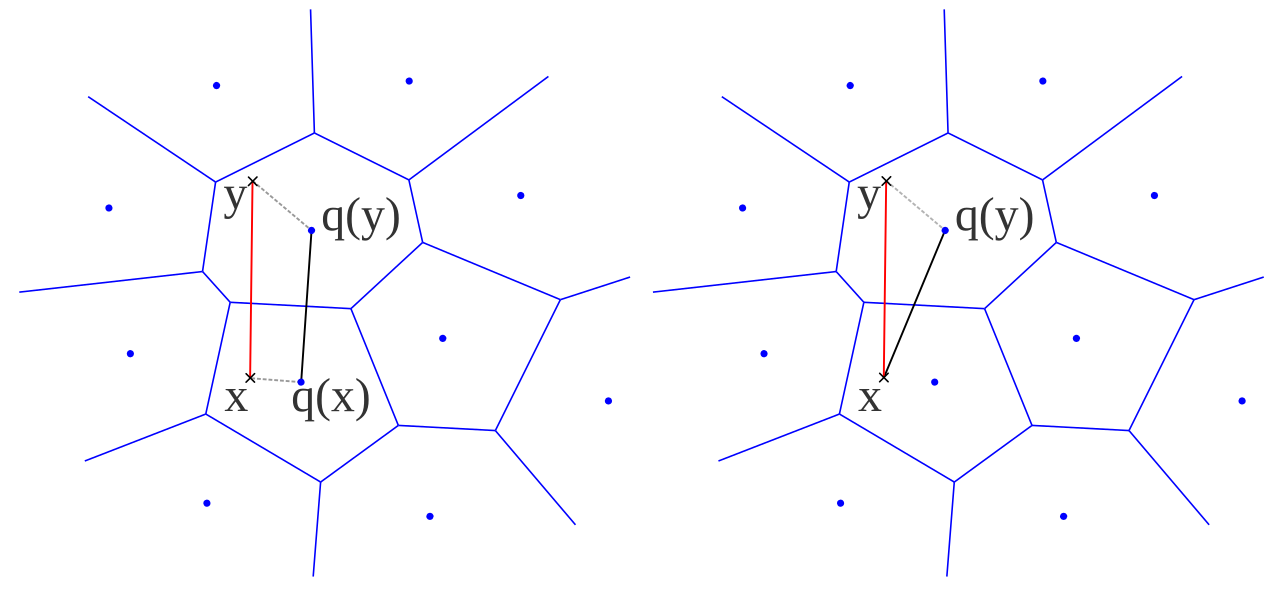
\includegraphics[width=1\linewidth]{Images/ADC_SDC.png}
\caption{Левый — симметричное расстояние. Правый — асимметричное расстояние. Расстояние $d(x,y)$ аппроксимируется расстоянием $d(q(x), q(y))$ и $d(x, q(y))$ для левого и правого рисунка соответственно.}
\label{ris:adc}
\end{figure}

\subsection{Вычисление расстояний}

Перед непосредственным описанием экспериментов опишем еще один важный момент. Рассмотрим вектор запроса $x$ и вектор индексированных данных $y$. Существует два метода вычисления приблизительного евклидова расстояния между этими векторами: симметричный и асимметричный (Рис.~\ref{ris:adc}).

Вычисление симметричного расстояния (SDC): оба вектора $x$ и $y$ представляются соответствующими центроидами $q(x)$ и $q(y)$. Расстояние $d(x, y)$ аппроксимируется расстоянием $d(x, y) = d(q(x), q(y))$, которое в случае многомерной индексации эффективно вычисляется следующим образом:
$$d(x, y) = d(q(x), q(y)) = \sqrt{\sum_{j=1}^M d(q_j(x),q_j(y))^2},$$
где расстояние между центроидами предварительно подсчитано. Справочная таблица каждого центроида содержит все квадраты расстояний до остальных центроидов.

Вычисление асимметричного расстояния (ADC): вектор $y$ представлен своим центроидом $q(y)$, а запрос $x$ не закодирован. Расстояние $d(x, y)$ аппроксимируется расстоянием $d(x, y) = d(x, q (y))$, которое вычисляется с использованием разложения:
$$d(x, y) = d(x, q(y)) = \sqrt{\sum_{j=1}^M d(x_j, q_j(y))^2)},$$
где $x_j$ — выделения компонент j-ой размерности мульти-индексного разбиения.

В обоих случаях функция корня обычно опускается. Единственное преимущество SDC перед ADC -- это меньшее использования памяти вектором запроса, поскольку он определяется своим кодом. В большинстве случаев это неактуально, поэтому используют асимметричную версию, которая позволяет получить меньшие искажения расстояния для аналогичной сложности. В остальной части работы используется ADC без явного упоминания.

\subsection{Эксперименты}

В данном разделе представлены описания экспериментов для каждой из исследуемых структур данных. Ограничимся здесь описанием основных принципов работы алгоритмов. Пошаговое описание работы каждой структуры представлено в следующем разделе.

Начнем с того, что для исследования поставленной задачи требуется огромное количество ресурсов. В связи с некоторыми ограничениями, будем проводить эксперименты на меньшем количестве данных и обобщать результат на общий случай исследования.

Для проведения экспериментов было обработано свыше 150 тысяч изображений. Для каждого из которых было произведено выделение лица и построение 128-мерного вектора признаков. Данные были сохранены в один csv-файл, который содержит информацию о 500 личностях.

Как упоминалось в постановке, нас интересует соотношения точности и скорости поиска для различных значений ближайших соседей ($K = 1, 5, 10, 30, 50, 100$). Время обучения структур не учитывается. Для чистоты экспериментов, все замеры проводятся по 1000 раз, затем результаты усредняются. На графиках ниже можно встретить две метрики точности <<Search>> и <<Recognition>>. Ломанная <<Search>> обозначает процент правильно найденных лиц среди $K$ ближайших соседей в одном запросе. Ломанная <<Recognition>> обозначает процент правильно распознанных людей во всех запросах, где успешным распознаванием считается совпадение лица запроса с лицом наибольшей частоты встречаемости среди $K$ ближайших соседей.

\subsubsection{Точный поиск}

Для сравнения результатов исследования проведем замеры точности поиска по евклидову расстоянию (Рис.~\ref{ris:euclidsearch}). Суть эксперимента в том, что данные не проходят предварительной обработки, а поиск происходит по всем имеющимся в базе данных векторам. Формируется общий ассоциативный список расстояний, который после сортировки показывает ближайшие к запросу вектора. Точность этого алгоритма будем считать эталонной, так как алгоритмы ANN не могут превысить точности исчерпывающего поиска.

\begin{figure}[h]
\begin{minipage}[h]{0.49\linewidth}
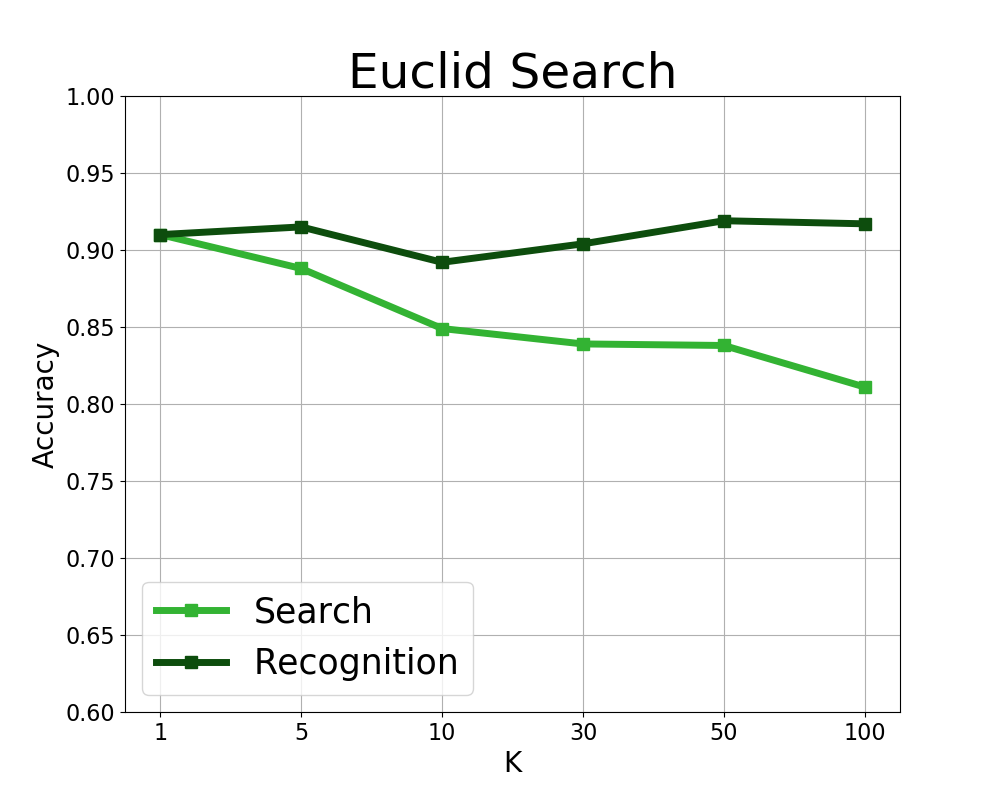
\includegraphics[width=1\linewidth]{Images/EuclidSearch.png}
\caption{Точность поиска по евклидову расстоянию.}
\label{ris:euclidsearch}
\end{minipage}
\hfill
\begin{minipage}[h]{0.49\linewidth}
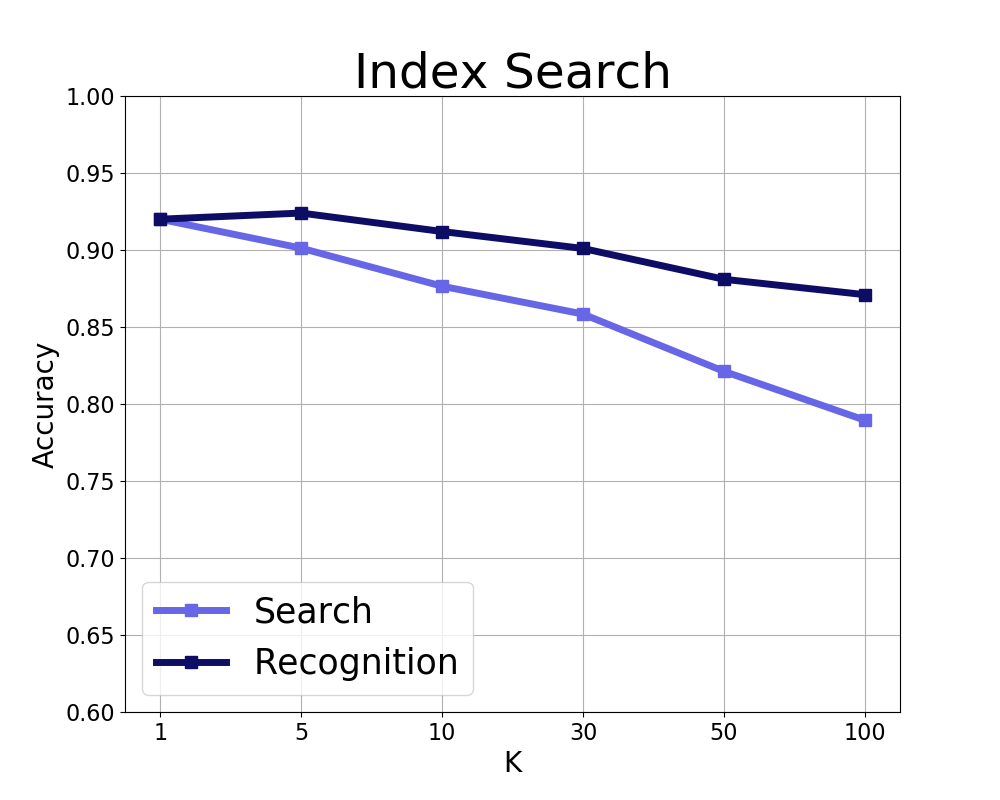
\includegraphics[width=1\linewidth]{Images/IndexSearch.png}
\caption{Точность поиска индексной структуры.}
\label{ris:indexsearch}
\end{minipage}
\end{figure}

Можно заметить и в чем мы убедимся позже, что вторая кривая находится в некоторой окрестности постоянного значения (0.90 -- 0.92). Это означает, что с расширением объема поиска процент лиц соответствующих запросу держится на одном уровне. <<Search>> кривая явно убывает, и связано это с тем, что при увеличении количества ближайших соседей вероятность попадания посторонних лиц в их число также увеличивается.

Перейдем к рассмотрению более продвинутых поисковых структур. Сначала сравним точность поиска и распознавания, а затем перейдем к оценке эффективности.

\subsubsection{Индексная структура}

Инвертированный индекс -- самый простой способ индексирования данных, но тем не менее даже он дает большой прирост в скорости поиска без ощутимого снижения качества. Для его использования требуется предобработка данных. Заметим, что из всех индексных структур, этот алгоритм требует наибольшего времени обучения, так как для построения индексной структуры используется классический алгоритм K-средних. Для исследуемых объемов данных он очень ресурсоемкий. Поиск по данной структуре разбивается на два этапа: 1) поиск ячейки; 2) поиск внутри ячейки. Для минимизации времени поиска требуется правильно подобрать параметры разбиения пространства. Путем поиска минимума функции $F(K)$ ($F(K)$ - общее количество вычислений расстояния), добиваемся оптимальной сложности поиска:
\begin{equation}\label{eq:index}
F(K)=K + \frac{N}{K},
\end{equation}
где $N$ -- объем базы данных, $K$ -- размер разбиения. 

Результаты исследования индексной структуры (Рис.~\ref{ris:indexsearch}) дают похожую картину точности, за тем лишь исключением, что общий показатель точности распознавания несколько упал (0.88 -- 0.91). Теперь при увеличении количества ближайших соседей <<Search>> кривая убывает быстрее. Это связанно с тем, что ближайшие к запросу центроиды не всегда точно определяют истинных ближайших соседей. Рассмотрение большего количества смежных ячеек улучшит результат, но негативно скажется на скорости поиска.

\begin{figure}[h]
\begin{minipage}[h]{0.49\linewidth}
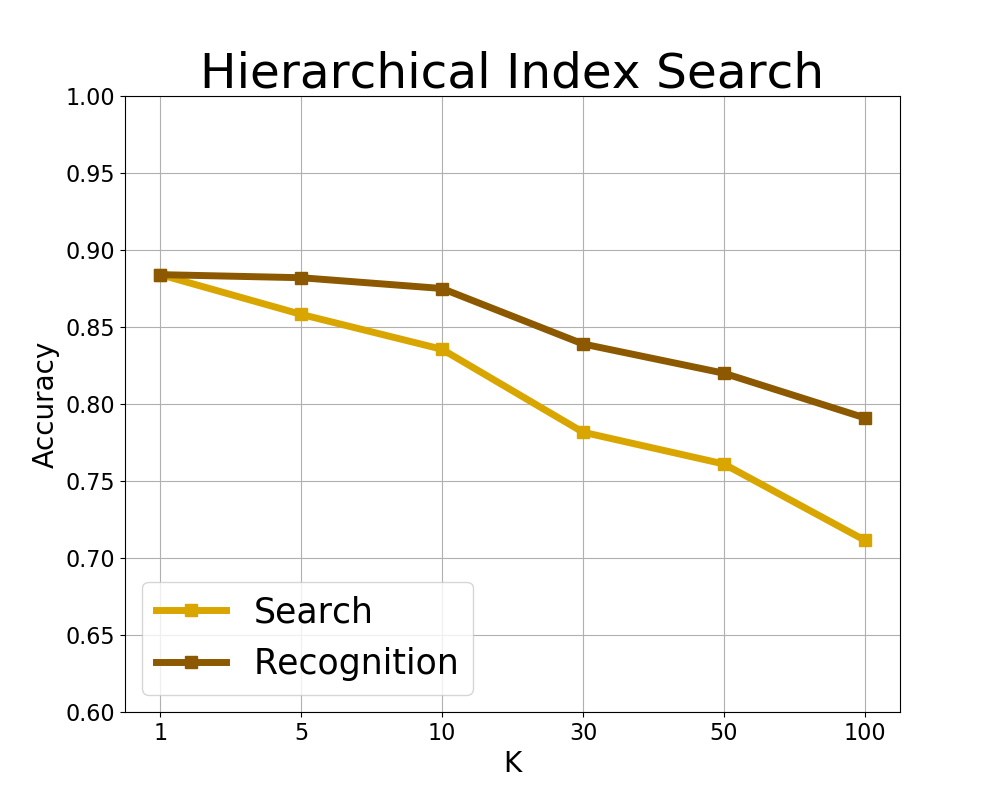
\includegraphics[width=1\linewidth]{Images/HierarchicalIndexSearch.png}
\caption{Точность поиска иерархической индексной структуры.}
\label{ris:hierarchicalindexsearch}
\end{minipage}
\hfill
\begin{minipage}[h]{0.49\linewidth}
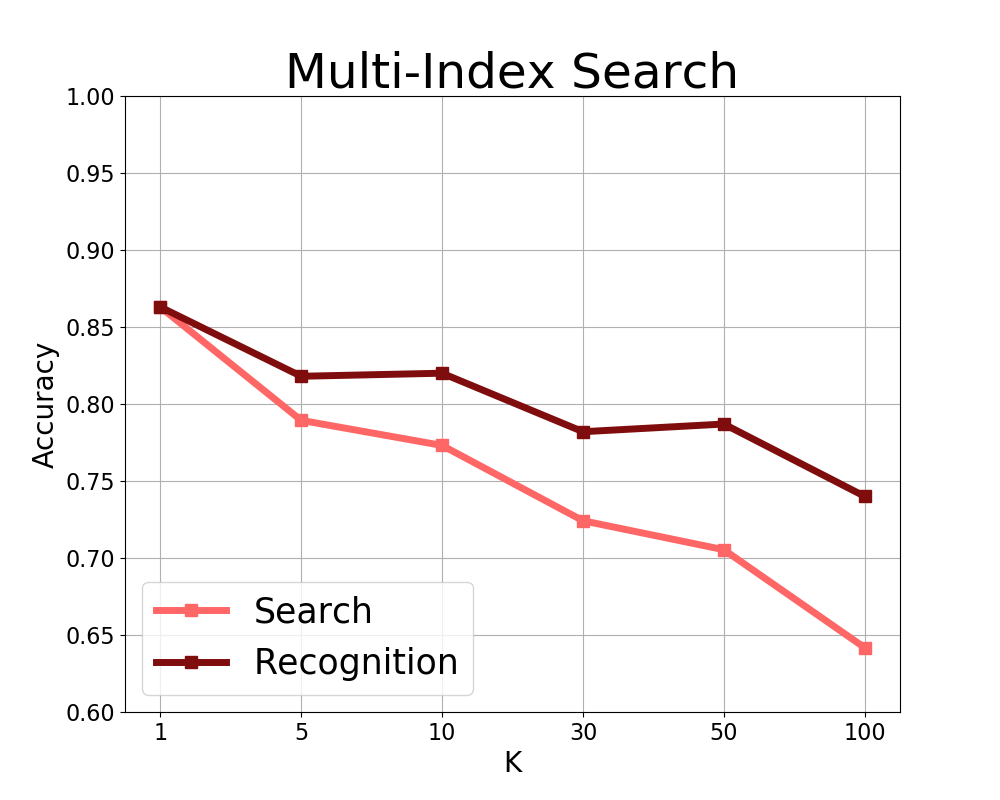
\includegraphics[width=1\linewidth]{Images/MultiIndexSearch.png}
\caption{Точность поиска мульти-индексной структуры.}
\label{ris:multiindexsearch}
\end{minipage}
\end{figure}

\subsubsection{Иерархическая структура}

Еще более существенно снизить количество вычислений помогает иерархический индекс. Этап предобрабтки для него схож с предыдущей структурой. Однако обучение происходит в несколько этапов: первичное разбиение и разбиение внутри каждой ячейки. Несмотря на большую запутанность алгоритма, обучается он на порядок быстрее. Связанно это с тем, что обучающий алгоритм существенно зависит от количества ячеек разбиения. Совокупное число ячеек здесь больше, но на каждом уровне обучения их оказывается меньше. Поиск по данной структуре тоже усложняется: 1) поиск ячейки первого уровня; 2) поиск ячейки второго уровня; 3) поиска внутри ячейки. Снова найдем минимум функции общего количества вычислений расстояния:
\begin{equation}\label{eq:hierachicalindex}
F(K_1,K_2)=K_1 + K_2 + \frac{N}{K_1K_2},
\end{equation}
где $N$ -- объем базы данных, $K_1$ и $K_2$ -- размер разбиения первого и второго уровня соответственно. 

Как видно из графика (Рис.~\ref{ris:hierarchicalindexsearch}), точность распознавания снова упала (0.82 -- 0.83). Здесь же можно заметить, что при $K = 100$ процент правильно найденных людей, среди $K$ ближайших соседей $\approx70\%$. Это ставит под вопрос применимость данной структуры в реальных задачах.

\subsubsection{Мульти-индексная структура}

Наиболее сложный и эффективный алгоритм, рассматриваемый в рамках этой работы — инвертированный мульти-индекс. Принцип его работы уже был описан в разделе <<Обзор существующих решений>>. Напомним, что этот алгоритм основан на произведении квантизации (PQ). Суть в том, что вектор разбивается на M подвекторов, и к каждому подвектору применяется классический алгоритм индексации, используя при этом отдельный список центроидов. Как было доказано в~\cite{3}, наибольшей эффективности алгоритм достигает при разбиении на два подпространства. Поэтому будем полагать, что $M = 2$. Что касается скорости обучения, то тут она еще выше. Если считать, что пространство разбивается на $K$ ячеек, то обучаться приходится лишь на $\sqrt{K}$ центроидах.

\begin{figure}[h]
\begin{minipage}[h]{0.48\linewidth}
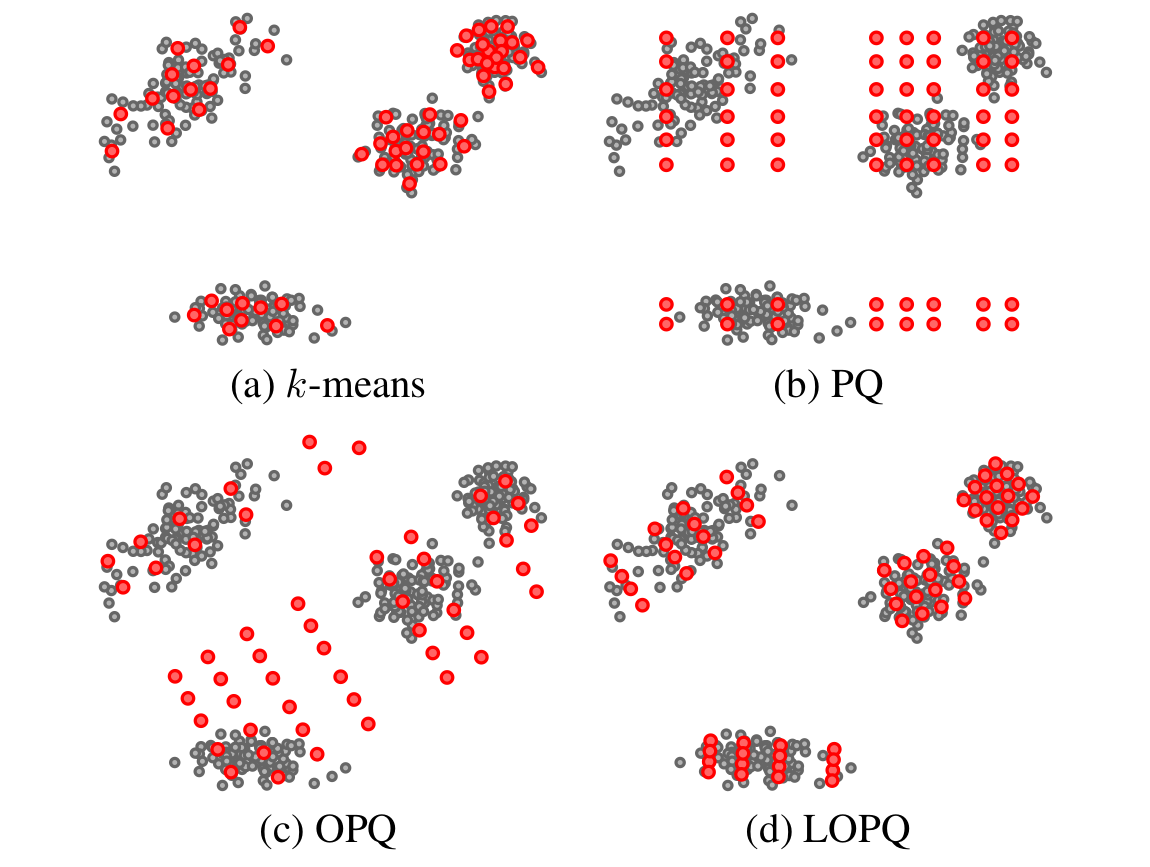
\includegraphics[width=1\linewidth]{Images/LOPQ.png}
\caption{Красными точками на рисунках обозначены центроиды. a) — инвертированный индекс; b) — инвертированный мульти-индекс; c) и d) — улeчшения мульти-индекса.}
\label{ris:lopq}
\end{minipage}
\hfill
\begin{minipage}[h]{0.48\linewidth}
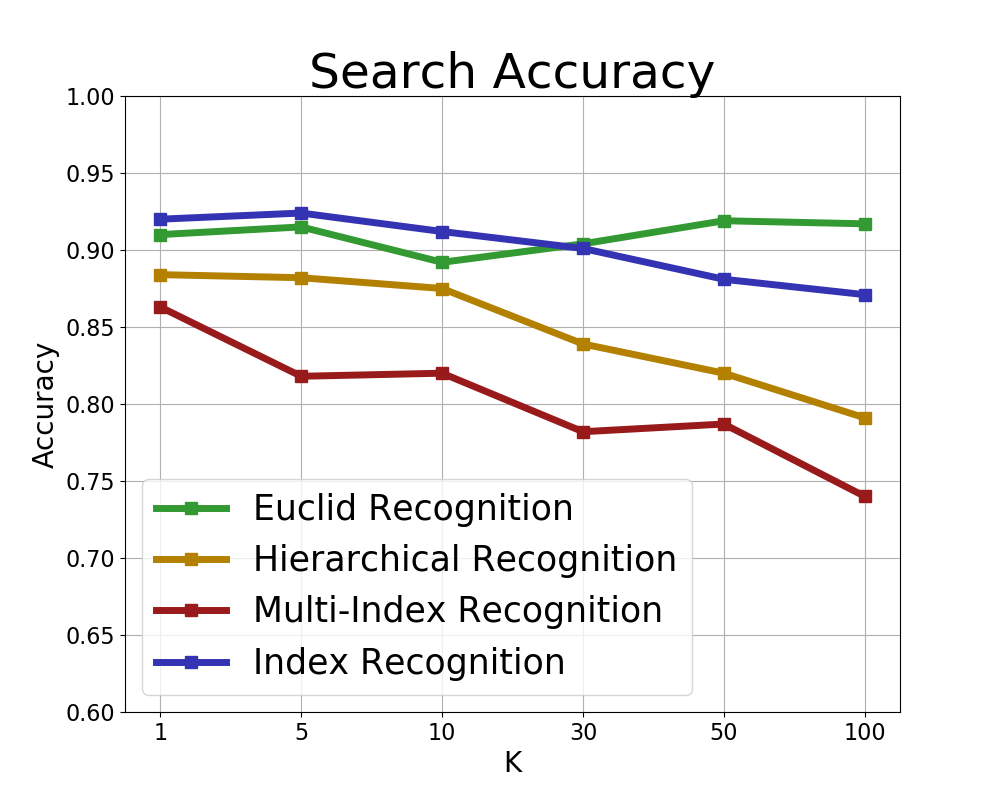
\includegraphics[width=1\linewidth]{Images/SearchAccuracy.png}
\caption{Сравнительный анализ точности поиска.}
\label{ris:searchaccuracy}
\end{minipage}
\end{figure}

Детальный алгоритм описан в следующем разделе, здесь лишь отметим, что для поиска соседей достаточно найти ближайшие центроиды всех подпространств запроса и взять их декартово произведение. Дабы снова избежать подбора параметров разбиения, найдем их оптимизацией следующей функции:
\begin{equation}\label{eq:multiindex}
F(K)= 2K + \frac{N}{K^2},
\end{equation}
где $N$ — объем базы данных, $K$ — размер разбиения каждого подпространства. 

На Рис.~\ref{ris:multiindexsearch} представлены измерения точности поиска мульти-индексной структуры. Из графика видно, что при больших значениях K показатели точности опускаются ниже $65\%$. Результат вполне очевидный, так как классическая реализация данного алгоритма показывает хороший результат только на равномерно распределенных данных, что неверно для нашего исследования. Поэтому стоит аккуратно относится к выбору этой структуры в реальных задачах.

Наглядное представление работы этих алгоритмов можно увидеть на Рис.~\ref{ris:lopq}. Здесь представлены два рассмотренных алгоритма, а также возможные пути улучшения последнего. Улучшения основаны на некоторой обработке векторов базы данных. Проблемы неравномерного распределения можно решить либо предварительным ортогональным преобразованием \cite{4,6}, либо локальными оптимизациям произведения квантизации \cite{5}.

На Рис.~\ref{ris:searchaccuracy} можно увидеть графики точности всех алгоритмов вместе. Здесь видны относительные показатели, которые позволяют сравнить алгоритмы друг с другом. Западение точности мульти-индексной структуры очевидно.

\begin{table}[h!]
\begin{tabular}{ | l | l | l | l | l | l | l | }
\hline
Алгоритм & $K = 1$ & $K = 5$ & $K = 10$ & $K = 30$ & $K = 50$ & $K = 100$  \\ \hline
Точный поиск & 0.395 & 0.339 & 0.365 & 0.347 & 0.326 & 0.343 \\
Индексная структура &0.00624 & 0.00806 & 0.00661 & 0.00687 & 0.00864 & 0.00827 \\
Мульти-индексная структура & 0.00212 & 0.00182 & 0.00211 & 0.00286 & 0.00284 & 0.00465 \\
Иерархическая структура & 0.00176 & 0.00182 & 0.00183 & 0.00151 & 0.00160 & 0.00156\\
\hline
\end{tabular}
\caption{Скорость поиска в секундах для различных значений $K$.}
\label{tab:results}
\end{table}

\begin{figure}[h]
\begin{minipage}[h]{0.49\linewidth}
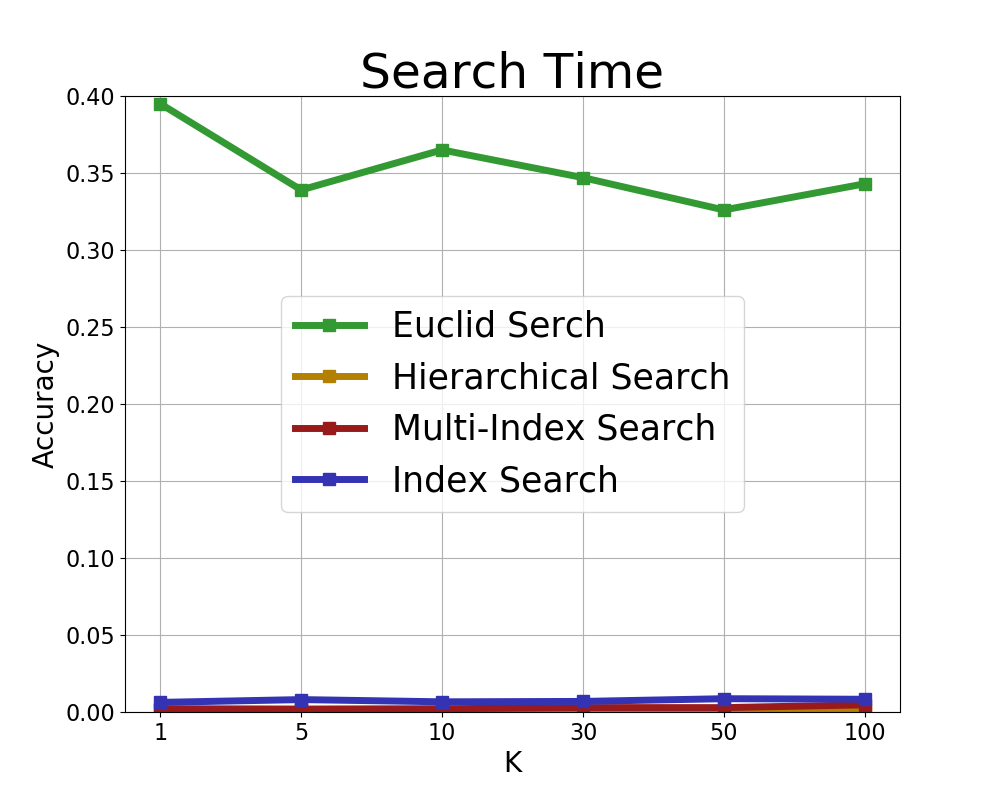
\includegraphics[width=1\linewidth]{Images/SearchTime.png}
\caption{Сравнительный анализ скорости поиска.}
\label{ris:searchtime}
\end{minipage}
\hfill
\begin{minipage}[h]{0.49\linewidth}
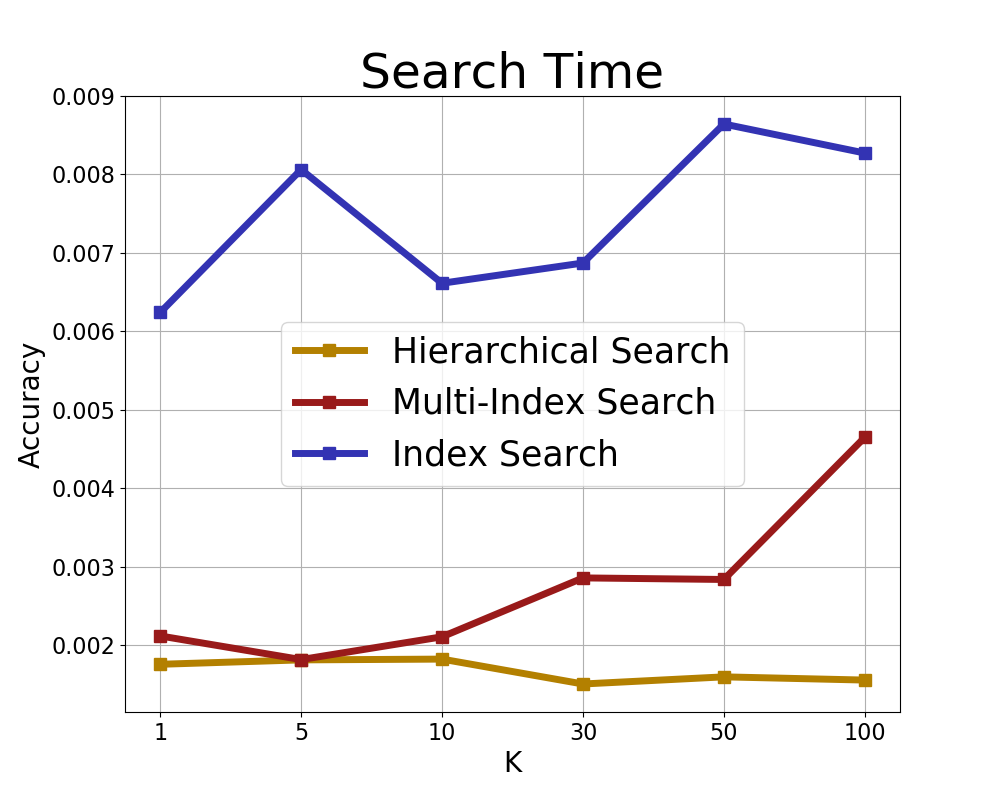
\includegraphics[width=1\linewidth]{Images/SearchTimeIndex.png}
\caption{Скорость поиска индексных структур.}
\label{ris:searchtimeindex}
\end{minipage}
\end{figure}

\subsection{Оценка времени поиска}

Теперь рассмотрим основной показатель эффективности этих структур данных. Время работы каждого запроса измерялось стандартными средствами языка программирования C++. Отсчет времени происходил с момента первого сравнения до последней сортировки кандидатов. В Таблице~\ref{tab:results} приведены численные значения результатов измерения времени. Для более наглядной оценки результатов приведен график зависимости времени поиска от $K$ (количество ближайших соседей) (Рис.~\ref{ris:searchtime}). Легко заметить, что любая индексная структура ускоряет поиск в сотни раз по сравнению с исчерпывающим поиском. На Рис.~\ref{ris:searchtimeindex} изображены ломанные соответствующие времени поиска только индексных структур для различных значений K ближайших соседей. Основная тенденция ломанных идет на возрастание, что связанно с тем, что при увеличении количества ближайших соседей также увеличивается список кандидатов. Резкие скачки на графике объясняются опять же неравномерностью распределения данных. % Исследование и построение решения задачи
\section{Описание практической части}
\label{sec:Chapter4} \index{Chapter4}

В данном разделе работы приведены обоснования использования тех или иных технологий и инструментов, а также оценена сложность используемых алгоритмов.

Для написания кода в этой работе используются два языка программирования: Python и C++. Весь код, который участвует в экспериментах написан на C++, так как известно преимущество в скорости этого языка, по сравнению с Python. Фрагменты программы для обучения структур распараллеливались с помощью технологии OpenMP. Как было сказано с предыдущем разделе, для обработки изображений была выбрана библиотека языка Python facerecognition. В связи с этим все скрипты подготовки набора данных были написаны на Python. 

Теперь рассмотрим более подробно каждый метод из предыдущего раздела и опишем используемые для него алгоритмы и структуры данных. Будем полагать, что база данных состоит из $N$ векторов. Вектор $y$ — произвольный вектор из набора данных, вектор $x$ — вектор запроса на поиск.

\subsection{Индексная структура}

Для обучения индексной структуры используется классический алгоритм кластеризации $K$-средних. Основная идея этого алгоритма заключается в том, что данные произвольно разбиваются на кластеры, после чего для каждого из них итеративно перевычисляется новый центр масс, затем векторы снова разбиваются на кластеры в соответствии с тем, какой из новых центров оказался ближе. Временная сложность работы алгоритма $K$-средних имеет следующую оценку: 
\begin{equation}\label{eq:kmeans}
O(IKND),
\end{equation}
где $I$ — число итераций обучения, $K$ — размер разбиения, $N$ — размер базы данных, $D$ — размерность векторов. Параметры $D$ и $N$ обсуждались ранее. Что касается параметра $I$, он был подобран опытным путем. На каждой итерации выводилась общая ошибка кластеризации $E$, и когда $\Delta E$ становилось достаточно мало, фиксировалось текущее значение $I$. Параметр $K$ находится путем оптимизации функции (\ref{eq:index}). Учитывая объем нашей задачи, получаем огромные затраты по времени на обучение алгоритма. Для ускорения этого этапа используется технология параллельного программирования OpenMP.

Поиск по данной структуре можно описать следующей последовательностью действий:
\begin{enumerate}
\item Вычисление расстояний от вектора запроса $x$ до векторов из списка центроидов. Сложность этого этапа оценивается как $O(KD)$;
\item Формирование списка кандидатов для завершающего поиска. Данный список формируется путем добавления в него векторов из ближайшего и смежных с ним кластеров. Причем кластеры выбираются в порядке наименьшего расстояния до запроса. Этот этап требует сортировки $K$ элементов;
\item Вычисление расстояний от $x$ до каждого вектора-кандидата. В зависимости от длины списка кандидатов, изменяется временная сложность вычислений. Гарантируется, что длина списка кандидатов не превышает заданного фиксированного значения;
\item Cортировка списка кандидатов по расстоянию до $x$.
\end{enumerate}

\subsection{Иерархическая структура}

Обучение иерархической и индексной структур в целом схожи. Однако первая проходит два цикла алгоритма $K$-средних. Связано это с тем, что помимо первого разбиения на кластеры, каждая ячейка разбивается повторно тем же алгоритмом. Суммарная сложность обучения оценивается как две сложности (\ref{eq:kmeans}) с параметрами $K_1$ и $K_2$ , которые являются решением задачи оптимизации функции (\ref{eq:hierachicalindex}). Во втором цикле обучения участвует в среднем $\frac{N}{K_1}$ векторов. Для ускорения обучения так же используется технология OpenMP. 

Приближенный поиск ближайших соседей в данной структуре включает следующие этапы:
\begin{enumerate}
\item Поиск ближайшего к вектору $x$ центроида в списке центроидов первичного разбиения. Сложность этого этапа оценивается как $O(K_1D)$;
\item Вычисление расстояний от вектора запроса x до векторов из списка вторичных центроидов, соответствующих первичному центроиду. Сложность этого этапа оценивается как $O(K_2D)$;
\item Формирование списка кандидатов для завершающего поиска. Данный список формируется из ячеек вторичного разбиения и, так же как и в индексной структуре, требует сортировки $K_2$ элементов;
\item Вычисление расстояний от $x$ до каждого вектора-кандидата. Сложность аналогична предыдущей структуре;
\item Cортировка списка кандидатов по расстоянию до $x$.
\end{enumerate}

\subsection{Мульти-индексная структура}

Для обучения мульти-индексной структуры так же применяется алгоритм $K$-средних. Однако теперь обучение проходит на векторах размерности $\frac{D}{2}$. В связи с этим общая сложность обучения может быть представлена как $2 * O(IKN\frac{D}{2})$. В данном случае K является аргументом минимизации функции (\ref{eq:multiindex}). Еще одна особенность обучения состоит в том, что после этого этапа на выходе формируется два независимых списка центроидов. И снова независимые по данным циклы распределяются по нескольким потокам.

Поиск по данной структуре описывается следующей последовательностью действий:
\begin{enumerate}
\item Вычисление расстояний от первой половины вектора $x$ до векторов из первого списка центроидов. Сложность $O(K\frac{D}{2})$;
\item Вычисление расстояний от второй половины вектора x до векторов из второго списка центроидов. Сложность $O(K\frac{D}{2})$;
\item Формирование приоритетной очереди ячеек кандидатов. Данный этап сортирует списки расстояний из пунктов 1. и 2. Затем декартово произведение ячеек первого и второго разбиения добавляются в приоритетную очередь, где в качестве приоритета выступает сумма расстояний до запроса $x$;
\item Формирование списка кандидатов. Из приоритетной очереди выбираются элементы максимального приоритета, и соответствующие им вектора добавляются в список кандидатов;
\item Cортировка списка кандидатов по расстоянию до $x$.
\end{enumerate} % Описание Экспериментальной части
\section*{Заключение}
\addcontentsline{toc}{section}{Заключение}
\label{sec:Chapter5} \index{Chapter5}
В рамках данной работы были исследованы современные индексные структуры быстрого поиска информации в больших объемах данных, а также проверена эффективность этих структур в задаче распознавания лиц. В результате экспериментов было выяснено, что при использовании любой из индексных структур скорость поиска возрастает в сотни раз по сравнению с исчерпывающим поиском. Временные затраты поиска в иерархической и мульти-индексной структурах находятся в окрестности нескольких миллисекунд, что согласуется с постановкой. Как и ожидалось, в ANN алгоритмах точность поиска начинает падать. При наивном использовании мульти-индексной структуры, точность поиска существенно снижается, что делает невозможным применение данного алгоритма на практике. Однако некоторые виды предобработки данных способны решить эту проблему. По точности и времени распознавания иерархическая структура оказалась наиболее универсальной.

Подводя итоги, приходим к выводу: в больших коллекция изображений лиц индексные структуры могут показать приемлемую скорость поиска с хорошим показателем точности, что дает им право использоваться в реальных задачах распознавания. % Заключение

\nocite{*}
\bibliographystyle{gost71u}
\bibliography{references}


\end{document}
